\chapter{Applied Nuclear Physics}
    \section{Nuclear Reactors}
        \href{https://www.youtube.com/watch?v=gGJKevXzN9A&list=RDCMUCIVaddFslWk1TFoKNrvh99Q&index=20}{Good Principles Video}
        \subsection{Obtaining sources}
            How is uranium enriched
        \subsection{Nuclear Reactor Startup}
            Video \href{https://en.wikipedia.org/wiki/Startup_neutron_source}{here}.
            
            
    \section{Nuclear Weapons}
    
    \section{Medicine}
        technetium-99
        
    \section{Other Nuclear Applications and Related}
        \subsection{How Do X-Ray Scans Work?}
            \indent Vacuum tube with 20 - 100 kV potential. Electrons emitted from cathode, accelerated, hit tungsten (Z=74) anode, produces x-rays through bremmstrahlung. Aluminum plate placed on output of x-ray source to absorb low-energy x-rays. Photographic plate beneath patient to absorb x-rays for imaging. X-ray sensitive film is usually an emulsion-gelatin containing silver halide crystals (silver bromide AgBr or silver chloride AgCl) on a transparent base. Coating is usually 10 micrometers thick. 
            
            For more info, see \href{https://www.youtube.com/watch?v=nSivTK6Icu4}{here}. 
            
        \subsection{How Do Computed Tomography (CT) Scans Work?}
            \indent Gives a 3D image of a body in the following way:\\
            \indent Patient sits on a bed, an xray source and photographic plate align across the patient. This source rotates around the patient, and the computer divides images up into voxels. By using math, we can get a 3D image of the person. For more information, see \href{https://www.youtube.com/watch?v=BmkdAqd5ReY}{here} and \href{https://www.youtube.com/watch?v=9SUHgtREWQc}{here}.
            
        \subsection{How Does Magnetic Resonance Imaging (MRI) Work?}
            \indent Hydrogen - proton plus electron. NMR only cares about the proton (nucleus) which has intrinsic rotation (spin). Humans are 70\% water, so have many hydrogen molecules. Fat and carbohydrates also have a lot of hydrogen. In general, humans have all spins averaged out, and are not magnetic. When humans go into a strong magnetic field, most spins align with the magnetic field, some align anti-parallel to magnetic field, in either a high or low energy state. These spins process around the axis, with a Larmor frequency. The frequency is 42.6 MHz per Tesla. A net magnetization is created pointing in the direction of the field. Then we inject a 42.6 MHz radio signal into the system, causing spin flips such that there is no longitudinal magnetization, and makes the spins resonate, so there is a transverse magnetization. This can be measured as it is an alternating magnetic signal, so induces an AC current. Because hydrogen atoms in water and in fat or carbohydrates have a different local structure, they give different signals for these processes, which can be mapped into 3D images. 
                        
            \begin{figure}[H]
    			\centering
    			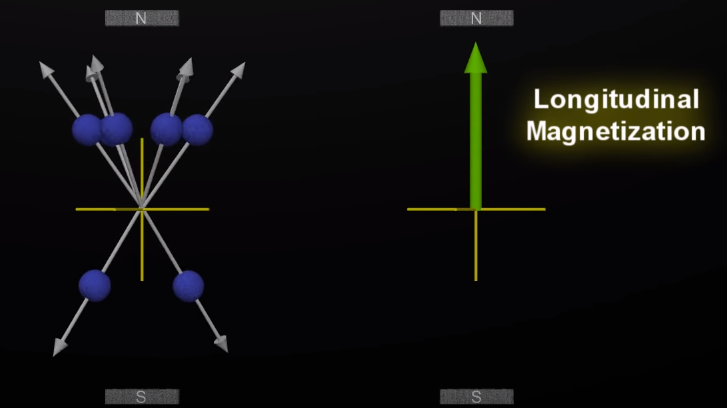
\includegraphics[width=12cm]{NuclearPhysics/modules/applied-nuclear/pics/mri-1.PNG}
    			\caption{MRI - 1}
    		\end{figure}
            
            \begin{figure}[H]
    			\centering
    			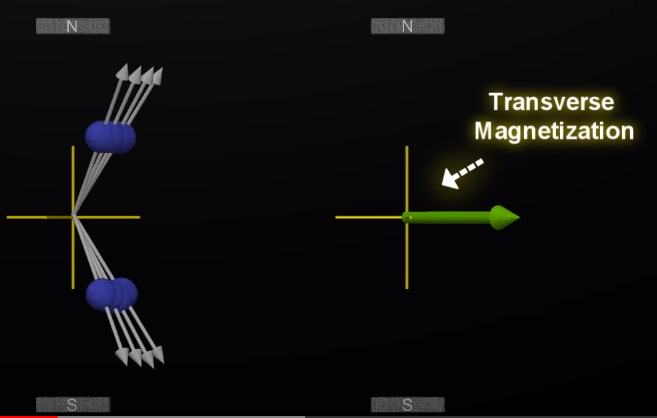
\includegraphics[width=12cm]{NuclearPhysics/modules/applied-nuclear/pics/mri-2.PNG}
    			\caption{MRI -2}
    		\end{figure}
            
            \begin{figure}[H]
    			\centering
    			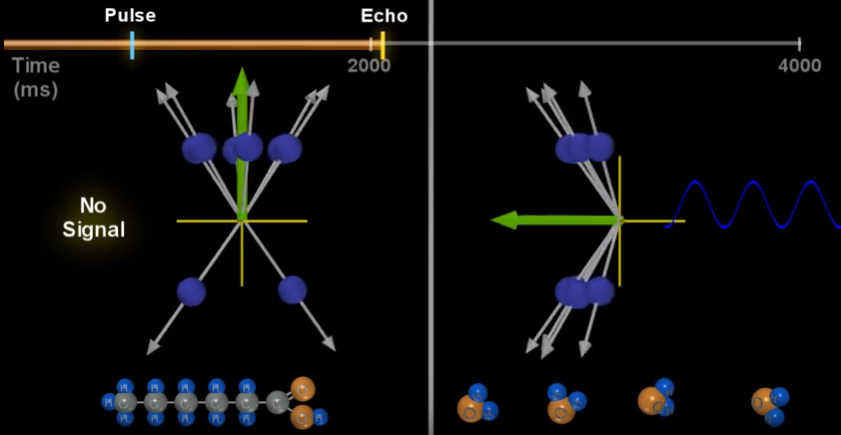
\includegraphics[width=12cm]{NuclearPhysics/modules/applied-nuclear/pics/mri-fat-water.PNG}
    			\caption{MRI - fat - water}
    		\end{figure}
    		
    		 \begin{figure}[H]
    			\centering
    			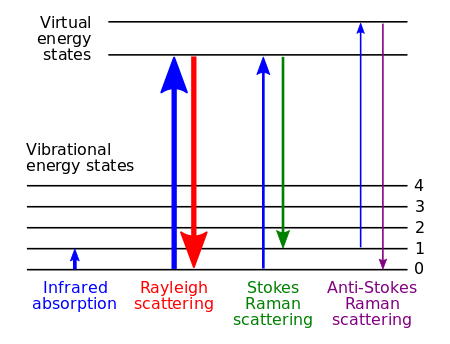
\includegraphics[width=12cm]{NuclearPhysics/modules/applied-nuclear/pics/raman.png}
    			\caption{Raman Spectroscopy}
    		\end{figure}
            
            More information here: \href{https://www.youtube.com/watch?v=djAxjtN_7VE}{video}\\
            Fun fact - the only reason MRI is not called NMR is because it came out during the Cold War, and patients would be hesitant to undergo any kind of "nuclear" treatment. 


        \myquantities{43 keV - energy of rotational state in Uranium}
        \myquantities{1.32 MeV - energy of vibrational state in Tin}
        \myquantities{8 MeV - binding energy of proton in lead }
        
        \subsection{What is Raman Spectroscopy}
            \indent Technique used to determine vibrational and rotational modes of molecules, commonly used in chemistry. Relies on inelastic scattering of photons, known as Raman scattering. Laser light of a specific frequency scatters inelastically off of phonons, causing the laser light to be shifted in energy up or down. This shift informs on the vibrational energy levels of the target.
            
            \href{https://www.youtube.com/watch?v=Gok7jRuer1k}{Raman Spectroscopy vid}
            \href{ttps://www.youtube.com/watch?v=_dPzIQEVEtc}{Another Raman Spec vid}
